Even if I did not personally fine-tuned BERT on SQuAD (I used DeepPavlov's pretrained BERT-SQuAD), in this subsection I will briefly outline the characteristics that made BERT a revolutionary model.

BERT, which stands for Bidirectional Encoder Representations from Transformers, is a new language representation model. Even if BERT was presented to the research world in May 2019, it has yet obtained new state-of-the-art results on eleven natural language processing tasks. For instance, a finetuned BERT push SQuAD v1.1 question answering F1 Test to 93.2 (1.5 points of absolute improvement) and SQuAD v2.0 F1 Test to 83.1 (5.1 points of absolute improvement).

The training framework proposed by Devlin et al., the authors of BERT, is composed of two steps: \textit{pre-training} and \textit{fine-tuning}. During pre-training BERT is trained over different pre-training tasks. The fine-tuning is only over a single downstream task, in our case, the SQuAD task.

BERT’s  model  architecture is a multi-layer bidirectional Transformer encoder. These last components, that are the building blocks of BERT, are implemented as described in the paper \textit{Attention Is All You Need} by Vaswani et al..

Considering BERT Base, the size taken in consideration for this project (the choice was between Base and Large), the hidden layers (i.e. Transformers encoders) are 12, the hidden size is 768 and the number of self-attention heads is 12.

\begin{figure}[t]
\centering
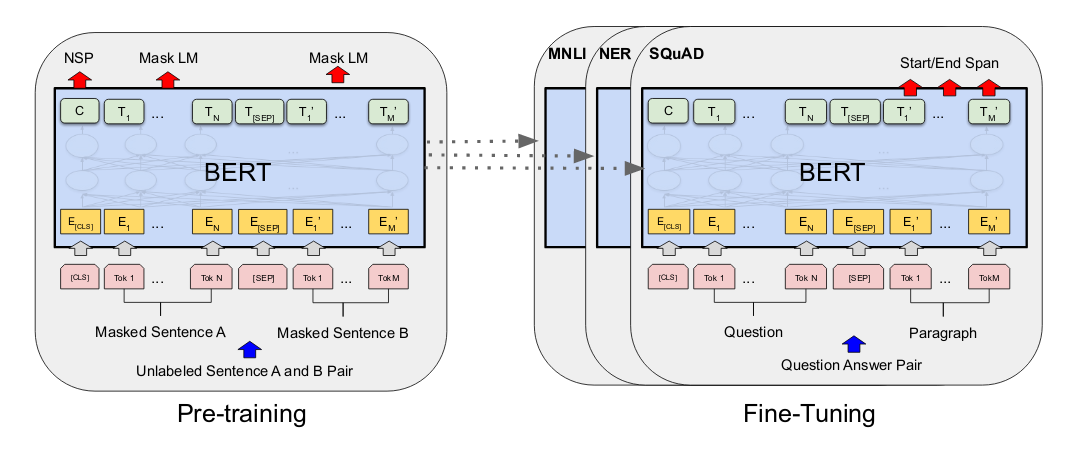
\includegraphics[width=18cm]{bert-for-squad-original-paper}
\caption{Overall pre-training and fine-tuning procedures for BERT. The pre-training procedure provides a basis for the numerous possible downstream tasks. \texttt{[CLS]}, which stands for ``classification'', is a special symbol added in front of every input example, and \texttt{[SEP]} is a special separator token. For further information about the input representation, please read the paper linked in bibliography (this image was taken by that paper).}
\medskip
\end{figure}

\subsubsection{Pre-training BERT}
Briefly, pre-training BERT means training it on two tasks:
\begin{itemize}
  \item \textit{Masked Language Model} (MLM), often called \textit{Cloze task}. A bidirectional model like BERT is undoubtedly more powerful than a left-context model like the OpenAI GPT Transformer. But this type of model is even more difficult to train because a bidirectional conditional language model cannot be trained left-to-right or right-to-left, since this would allow each word to indirectly “see itself” during training. Thus, in order to train a bidirectional representation, the researchers simply mask some percentage of the input tokens at random (15\% in their experiments), and then predict those masked tokens. Masking a tokens means substitute a real token with a placeholder token \texttt{[MASK]}. 
  \item \textit{Next Sentence Prediction} (NSP). This task is beneficial to many important downstream tasks like Question Answering and Natural Language Inference that are based on understanding the relation between two sentences, skill that is not captured by the previous task. Basically, this task is a binary \textit{next sentence prediction}: when choosing the sentences \texttt{A} and \texttt{B} for the training, in the 50\% of the cases \texttt{B} is an actual next sentence of \texttt{A} (and it is labeled as \texttt{IsNext}) while in the other cases the choice of \texttt{B} is random between the sentences (labeled as \texttt{NotNext}).
\end{itemize}

\subsubsection{Fine-tuning BERT: preparing it for Reading Comprehension}

Analizzare il fine-tuning di SQuAD 1.1, accennare solo al fatto che squad 2.0 puo' anche non rispondere alle domande.

$S \in \mathbb{R}^\mathbb{H}$

$E \in \mathbb{R}^\mathbb{H}$

$P_{i} = \frac{\mathrm{e}^{S \cdot T_{i}}}{\sum_{j} \mathrm{e}^{S \cdot T_{j}}}$

$score_{i, j} = S \cdot T_{i} + E \cdot T_{j}$

%% loglikelihood:

$loglikelihood(S) = \sum_{i} y_{i} \mathrm{ln} (P(y_{i} | S)) + (1 - y_{i}) \mathrm{ln} (1 - P(y_{i} | S))$